\documentclass{article}
\usepackage[utf8]{inputenc}
\usepackage[T1]{fontenc}
\usepackage[french]{babel}
\usepackage{graphicx}
\usepackage{fancyhdr}
\usepackage{geometry}
\usepackage{tabularx}
\usepackage{setspace}
\usepackage{blindtext}
\usepackage{pdfpages}
\usepackage{appendix}
\usepackage[none]{hyphenat}
\usepackage{xcolor}

\title{Rapport PPII : Démocratie Participative}
\author{Elion Hashani & Thibault Chenevière & Antoine Yebouet & Thom Guillot}
\date{December 2021}

\geometry{legalpaper, margin=1.5in}
\renewcommand*\contentsname{Table des matières}

\pagestyle{fancy}
\fancyhf{}
\rhead{Démocratie Participative}
\lhead{PPII}
\rfoot{Page \thepage}

\begin{document}

%Page de garde

\thispagestyle{empty}

\vskip 2cm

\begin{figure}[ht!]
    \centering
    
\includegraphics[scale = 0.11]{logoTNCY.png}
    \label{fig:logo_TNCY}
\end{figure}
\vskip 0.3cm
\begin{center}
\begin{LARGE}
TELECOM Nancy
\\
\vskip 2.7cm
Projet PPII
\end{LARGE}
\\
\vskip 2.7cm
\hline
\vskip 1.8cm
\begin{Huge}
\textbf{Démocratie Participative}
\end{Huge}
\vskip 1.8cm
\hline
\end{center}

\vskip 1.5cm

\begin{Large}
\noindent Cheneviere Thibault 
\hfill {} Responsables du module :\\
Guillot Thom 
\hfill{} Olivier Festor\\
Hashani Elion
\hfill{} Gerald Oster\\
Yebouet Antoine\\

\end{Large}

\vskip 1cm
\begin{figure}
    \centering
    
\includegraphics[scale = 1.8]{logo_UL.jpg}
\end{figure}

%Fin de la page de garde

\tableofcontents


\newpage
%Debut chapitre 1 : Introduction au sujet
\section{Introduction au sujet}
\vskip 0.60cm
\subsection{Contexte du projet}
\vskip 0.25cm
\noindent
Ce projet à été réalisé dans le cadre du module CS54 (Computer Science 54) de la première année du cycle ingénieur sous statut étudiant de TELECOM Nancy.
\vskip 0.25cm
\noindent
L'objectif de ce projet est d'utiliser nos connaissances des différentes sections du module (Algorithmique, Bases de données et Web) et de mettre en oeuvre les principes de gestion de projet appris dans le cours de gestion de projet pour concevoir une application Web sur le thème de la démocratie participative.
\vskip 0.25cm
\subsection{Organisation du document}
\vskip 0.25cm
\noindent
Dans le chapitre 2, nous ferons une présentation de la démocratie participative et la Civic Tech, et par un état de l'art, nous analyserons les applications existantes de Civic Tech.
\vskip 0.25cm
\noindent
Dans le chapitre 3, nous présentation la conception et l'implémentation de l'application Web, en présentant chacun des trois volets de l'application, bases de données, serveur web et algorithmes de traitement. 
\vskip 0.25cm
\noindent
Dans le chapitre 4, nous présenterons les tests réalisés dans notre application et les performances de cette dernière.
\vskip 0.25cm
\noindent
Dans le chapitre 5 nous présenterons les éléments et outils de gestion de projet que nous avons utilisé, puis dans le chapitre 6, nous ferons un Bilan du projet.
\vskip 0.25cm
\subsection{Principe de fonctionnement général de l'application}
\vskip 0.25cm
\noindent
L'application possède 3 grandes fonctionnalités :
\begin{itemize}
    \item Afficher de façon synthétique les différents candidats à l'élection
    \item Voir l'attention portée par les candidats aux thèmes pertinents pour une élection
    \item Renseigner le chemin le plus rapide vers le bureau de vote le plus proche
\end{itemize}
\vskip 0.25cm
\noindent
Pour ce faire, les candidats seront présentés sous forme de petites cartes constituant un bref résumé du candidat en question en affichant sa description, ses statistiques et le début de son programme. Ils sont ensuite répartis par parti politique afin d'avoir un critère de sélection en plus pour les visiteurs.
\vskip 0.25cm
\noindent
Les statistiques sont établies par analyse du programme du candidat et quantifient l'attention de celui-ci envers les thèmes suivants : Environnement, Social et Économie. Elles reposent sur un nombre de mots-clés présents (ou non) dans le programme.
\vskip 0.25cm
\noindent
De plus, chaque visiteur pourra porter un jugement sur les statistiques de chaque candidat après lecture du programme si le pourcentage déjà présent ne lui convient pas. Après un certain nombre d'avis allant dans le même sens, la statistique du candidat changera et ne pourra plus être modifiée.
\vskip 0.25cm

%Note à moi même : revoir et finir l'intro /!\
%Fin chapitre 1

\newpage
%Debut chapitre 2 : Etat de l'art
\section{État de l'art}
\subsection{Principe de la Civic Tech}
\vskip 0.25cm
\noindent
La Civic Tech est définie comme étant un outil au service de la démocratie participative. Cette technologie permet l'engagement ainsi que la participation des citoyens dans la décision publique. Avec une mise en relation des citoyens, la Civic Tech leur permet de s'engager auprès de leur gouvernement dans le but de travailler ensemble pour le bien public.
\vskip 0.25cm
\subsection{Analyse des exemples de Civic Tech}

\begin{tabularx}{\textwidth}{X|X|X|X|X}
    \color{blue}Application & \color{blue} Créateurs & \color{blue} But & \color{blue} Fonctionnalités & \color{blue} Lieu/Fréquence d'usage  \\
    \hline
    Consul & Mairie de Madrid avec Pablo Soto, développé en 2016 & Citoyens font remonter des idées aux mairies; campagne de budget participatif & Budget Participatif, Vote, Débat proposé par les utilisateurs, Pétition, Propositions & Vie de tous les jours et dans le monde entier mais principalement en Espagne \\
    \hline
    Assembl & Bluenove & Construire la prochaine constitution européenne avec les citoyens Européens,
    débats et consultations en ligne à grande échelle & Vote, Questionnaire, Débat proposé par les utilisateurs, Prise de décision & Europe et vie quotidienne avec cycle de débat sur 10 semaines.\\
    \hline
    DemocracyOS & Développeurs et politologues en Argentine & Accompagner et rassembler des mouvements citoyens, des institutions, des start-ups, des associations & Consultation publique, Vote, Proposition, Débat proposé par les utilisateurs, Prise de décision & L'application a été reprise dans le monde entier et utilisable à tout moment.\\
    \hline
    Maires\&Citoyens & Créée en 2016 par 2 azuréens & Épauler les maires et élus
    à communiquer efficacement et en temps réel avec les habitants de la commune & Alertes communales, sondages anonymes, suggestions citoyennes, signalements urbains et groupes de discussion & Près de 250 communes en France l'utilise et peut être utilisé quotidiennement\\
    \hline
    DigitaleBox & Fondée en 2013 par Vincent Moncenis & Logiciel de gestion des relations avec les électeurs et de stratégie électoralex & Gestion des réseaux sociaux, communications ciblées, organisation de communautés & En France, surtout utilisé lors des campagnes éléctorales\\
    \hline
    FluiCity & 	Julie de Pimodan \& Nicolas de Briey \& Jonathan Meiss & Facilite la mise en place de nos consultations citoyennes et renforce leur impact & Organiser des conseils, budget participatif, événement, signalement, proposition & Plus de 100 villes \& régions en France et en Belgique, peut être utilisé quotidiennement.\\
\end{tabularx}

\vskip 0.25cm
\subsection{Choix de notre application}
\vskip 0.25cm
\noindent
Suite à plusieurs brainstorming réalisés ainsi que des recherches Web, nous avons pu remarquer que notre société cherche à accéder aux informations de manière instantanée et guidée, avec un effor minimal. On observe une abstention des jeunes plus forte à chaque élection que ce soit pour les départementales, les régionales ou même les présidentielles. Il fallait ainsi que l'on trouve une approche adaptée à cette problématique.
\vskip 0.25cm
\noindent
C'est pour cela qu'une application, s'inspirant de la Civic Tech, permettant d'avoir des statistiques sur chaque candidat répondait à la problématique évoqué précédemment. Cette application est accessible à tous, ludique : avec le design des cartes résumant les candidats, ainsi que le système de vote qui permet de réévaluer les statistiques d'un candidat ; et permet aux utilisateurs de choisir le candidat, pour lequel ils vont voter, plus facilement selon leurs critères.
\vskip 0.25cm
%Fin chapitre 2

\newpage
%Debut chapitre 3 : Conception et implementation de l'application
\section{Conception et implémentation de l'application}
\vskip 0.60cm
\subsection{Introduction}
\vskip 0.25cm
\noindent
Pour la conception et l'implémentation de l'application, nous avons utilisé Visual Studio Code comme Environnement de développement. Nous avons utilisé le framework Flask pour le développement web, sqlite3 pour la base de données nous avons réalisé les algorithmes de traitement en Python. Nous avons aussi d'autres langages tels que JavaScript, HTML, CSS.
\vskip 0.25cm
\subsection{Base de données}
\vskip 0.25cm
\subsubsection{Modèle relationnel}
Voici le modèle relationnel de la base de données utilisée dans notre application :
\newline
\newline
\textbf{Exemple} : une table
\newline
\underline{   } : clé primaire
\newline
\# : clé étrangère
\newline
\newline
\textbf{Candidate}(\underline{id}, firstName, lastName, picture, catchphrase, \#listId, mail, job, identifier, password)
\newline
\textbf{List}(\underline{id}, name, program, politicalEdge)
\newline
\textbf{ProgramGrade}(\underline{id}, \#listId, environment, social, economy)
\newline
\textbf{Users\textunderscore vote}(\underline{id}, \#listId, userIP, economyVote, ecologyVote, socialVote)
\newline
\textbf{Member}(\underline{id}, firstName, lastName, \#listId, job)
\newline
\textbf{jobMemberGrade}(\underline{id}, \#listId, agriexp, artcomchef, cadreprofintsup, profintermed, employe, ouvrier, retraite, sansactprof)
\newline
\textbf{Vote\textunderscore office}(\underline{id}, lat, lon, name)

\subsubsection{Schémas relationnels et contraintes}
Voici le schéma relationnel de la base de donnée utilisé dans notre application :
\newline\newline

\noindent
CREATE TABLE Candidate
    \newline\indent\indent
    (
        \newline\indent\indent\indent
        id INTEGER PRIMARY KEY AUTOINCREMENT,
        \newline\indent\indent\indent
        firstName TEXT,
        \newline\indent\indent\indent
        lastName TEXT,
        \newline\indent\indent\indent
        picture TEXT,
        \newline\indent\indent\indent
        catchphrase TEXT,
        \newline\indent\indent\indent
        listId INTEGER,
        \newline\indent\indent\indent
        email TEXT UNIQUE,
        \newline\indent\indent\indent
        job TEXT,
        \newline\indent\indent\indent
        identifier TEXT UNIQUE,
        \newline\indent\indent\indent
        password TEXT,
        \newline\indent\indent\indent
        FOREIGN KEY (listId) REFERENCES List(id)
    \newline\indent\indent
    );
\newline\newline
CREATE TABLE List
    \newline\indent\indent
    (
        \newline\indent\indent\indent
        id INTEGER PRIMARY KEY AUTOINCREMENT,
        \newline\indent\indent\indent
        name TEXT,
        \newline\indent\indent\indent
        program TEXT,
        \newline\indent\indent\indent
        politicalEdge TEXT
    \newline\indent\indent
    );
\newline\newline
\newpage

CREATE TABLE ProgramGrade
    \newline\indent\indent
    (
        \newline\indent\indent\indent
        id INTEGER PRIMARY KEY AUTOINCREMENT,
        \newline\indent\indent\indent
        listId INTEGER,
        \newline\indent\indent\indent
        environment FLOAT,
        \newline\indent\indent\indent
        social FLOAT,
        \newline\indent\indent\indent
        economy FLOAT,
        \newline\indent\indent\indent
        FOREIGN KEY (listId) REFERENCES List(id)
    \newline\indent\indent
    );
\newline\newline
CREATE TABLE Member
    \newline
    \indent\indent
    (
        \newline
        \indent\indent\indent
        id INTEGER PRIMARY KEY AUTOINCREMENT,
        \newline
        \indent\indent\indent
        firstName TEXT,
        \newline
        \indent\indent\indent
        lastName TEXT,
        \newline
        \indent\indent\indent
        listId INTEGER,
        \newline
        \indent\indent\indent
        job TEXT,
        \newline
        \indent\indent\indent
        FOREIGN KEY (listId) REFERENCES List(id)
    \newline
    \indent\indent
    );
\newline\newline
CREATE TABLE Users\textunderscore vote
    \newline\indent\indent
    (
        \newline\indent\indent\indent
        id INTEGER PRIMARY KEY AUTOINCREMENT,
        \newline\indent\indent\indent
        listId INTEGER,
        \newline\indent\indent\indent
        userIP TEXT NOT NULL,
        \newline\indent\indent\indent
        economyVote INTEGER DEFAULT 0,
        \newline\indent\indent\indent
        ecologyVote INTEGER DEFAULT 0,
        \newline\indent\indent\indent
        socialVote INTEGER DEFAULT 0,
        \newline\indent\indent\indent
        FOREIGN KEY (listId) REFERENCES List(id)
    \newline\indent\indent
    );
\newline\newline
CREATE TABLE Vote\textunderscore office
    \newline\indent\indent
    (
        \newline\indent\indent\indent
        id INTEGER PRIMARY KEY AUTOINCREMENT,
        \newline\indent\indent\indent
        lat FLOAT NOT NULL,
        \newline\indent\indent\indent
        lon FLOAT NOT NULL,
        \newline\indent\indent\indent
        name TEXT NOT NULL
    \newline\indent\indent
    );
\newline\newline
CREATE TABLE jobMemberGrade
    \newline\indent\indent
    (
        \newline\indent\indent\indent
        id INTEGER PRIMARY KEY AUTOINCREMENT,
        \newline\indent\indent\indent
        listId INTEGER NOT NULL,
        \newline\indent\indent\indent
        agriexp INTEGER DEFAULT 0,
        \newline\indent\indent\indent
        artcomchef INTEGER DEFAULT 0,
        \newline\indent\indent\indent
        cadreprofintsup INTEGER DEFAULT 0,
        \newline\indent\indent\indent
        profintermed INTEGER DEFAULT 0,
        \newline\indent\indent\indent
        employe INTEGER DEFAULT 0,
        \newline\indent\indent\indent
        ouvrier INTEGER DEFAULT 0,
        \newline\indent\indent\indent
        retraite INTEGER DEFAULT 0,
        \newline\indent\indent\indent
        sansactprof INTEGER DEFAULT 0,
        \newline\indent\indent\indent
        FOREIGN KEY (listId) REFERENCES List(id)
    \newline\indent\indent
    );
\newline\newline
Pour le schema de la base de donnée voir figure \ref{fig:schemaBD}
\begin{figure}
    \centering
    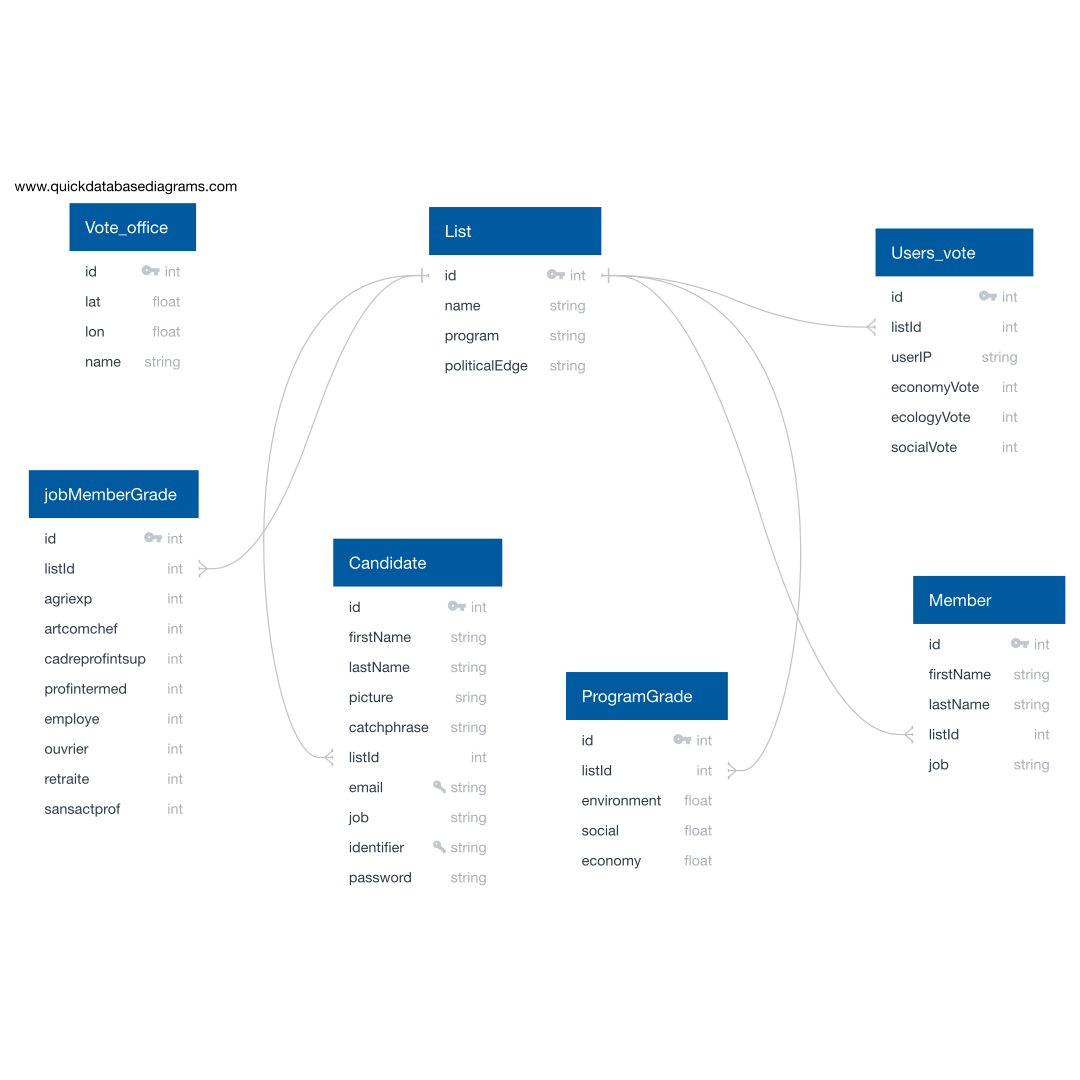
\includegraphics[scale = 0.4]{schemaBD_PPII.png}
    \caption{Schema de la base de donnée}
    \label{fig:schemaBD}
\end{figure}
\newpage

\subsubsection{Implémentation de la base de données}
\vskip 0.25cm
\noindent
Nous avons utilisé le module pysqlite3 afin d'accéder à la base de données directement dans nos fonctions de traitement des données. Quelques fonctions sont dédiées à la manipulation des données directement dans les tables comme \textit{alterDatabase.py} et permettent ainsi de faciliter l'ajout des différents candidats et de leurs identifiants de connexion.
\vskip 0.25cm
\subsection{Serveur Web}
\subsubsection{Général}
\vskip 0.25cm
\noindent
Le site est composé de 4 pages web accessibles par tous les visiteurs et possède 2 pages web accessibles par les utilisateurs qui possèdent un identifiant : les candidats.
\vskip 0.25cm
\noindent
Toutes les pages possèdent la même barre de navigation et le même pied de page. La barre de navigation diffère selon l'utilisateur et affiche uniquement les pages accessibles par ceux-ci. Le pied de page possède un lien vers chaque réseaux sociaux spécifiques à la page et un lien vers la page de Télécom Nancy. Le style des pages est géré par un layout et majoritairement du Bootstrap 5 pour quelques modifications en CSS.
\vskip 0.25cm
\subsubsection{Page d'accueil}
\vskip 0.25cm
\noindent
Le visiteur est accueilli par cette page sur le site et peut accéder à deux sections :
\begin{itemize}
    \item Comment ça marche ?
    \item Liste des candidats
\end{itemize}
\vskip 0.25cm
\noindent
Les routes menant à cette page sont \textit{'/'} et \textit{'/home'} (la route \textit{'/home'} est utilisée lorsqu'on clique sur le premier onglet dans la barre de navigation).
\vskip 0.25cm
\noindent
La première section explique le fonctionnement du site et est affichée en priorité à chaque visite de cette page. La deuxième section est à l'origine cachée et affiche la liste des candidats sous forme de cartes en fonction de leur parti politique dans les listes déroulantes correspondantes. L'affichage de ces deux sections est régulé en JavaScript afin de n'afficher qu'une seule section à la fois.
\vskip 0.25cm
\subsubsection{Carte des bureaux de vote}
\vskip 0.25cm
\noindent
Cette page affiche une carte et un itinéraire vers le bureau de vote le plus proche de l'utilisateur (les bureaux de vote sont répertoriés dans la base de données). Elle est accessible par la route \textit{'/map'}. L'utilisateur a le choix de trois moyens de transport : vélo, voiture et marche. L'API pour la carte et l'itinéraire est "mapbox" et permet donc d'avoir cette fonctionnalité de meilleur itinéraire.
\vskip 0.25cm
\subsubsection{Programme d'un candidat}
\vskip 0.25cm
\noindent
Chaque candidat possède une page plus grande que les petites cartes présentes sur la page d'accueil afin d'y afficher notamment son programme dans son intégralité, les membres de sa liste électorale et leur catégorie socio-professionnelle. Cette page est accessible grâce à la route \textit{'/program/(Prénom)/(Nom)/(Id dans la base de données)'} ce qui permet un affichage de la page spécifique à chaque candidat.
\vskip 0.25cm
\noindent
Cette page contient la fonctionnalité principale du site qui est de "noter" les programmes de chaque candidat en influant sur le pourcentage d'attention apporté aux thèmes principaux (Environnement, Social, Économie).
\vskip 0.25cm
\subsubsection{Connexion}
\vskip 0.25cm
\noindent
La page de connexion permet aux candidats d'accéder aux pages qui leur sont spécifiques pour pouvoir référencer leur programme, leur liste électorale et ajouter différentes informations pour compléter leur profil. Elle est accessible grâce à la route \textit{'/login'}. Seuls les candidats ont accès à des identifiants attribués par un gérant du site.
\vskip 0.25cm
\subsubsection{Profil de l'utilisateur}
\vskip 0.25cm
\noindent
Le profil est accessible uniquement lorsque l'on est connecté sur le site et la route suit le même principe que la route pour la page du programme d'un candidat \textit{'/profile/(Prénom)/(Nom)/(Id dans la base de données)'}. On peut y rentrer une citation et y mettre une photo de profil.
\vskip 0.25cm
\subsubsection{Référencement du programme}
\vskip 0.25cm
\noindent
Les candidats ont accès à une page afin d'y renseigner leur programme et les membres de leur liste électorale avec leur catégorie socio-professionnelle. La route d'accès pour cette page est \textit{'/defineProgram'}. La page est donc divisée en deux sections et affichent les membres déjà renseignés et le programme s'il est déjà écrit afin de le modifier à souhait.
\vskip 0.25cm
\subsection{Algorithmes de traitement}
\vskip 0.25cm
\subsubsection{Introduction}
\vskip 0.25cm
\noindent
Les algorithmes implémentés ont permis de faciliter la récupération et le traitement des données acquises via des requêtes dans la base de données afin de les réinjecter dans les pages HTML par la suite. Certains agorithmes s'occupent simplement de séparer des données, mais d'autres permettent d'introduire de nouvelles données dans (\textit{database.db}) en vue d'être utilisées ensuite sur une page web comme les statistiques par thème de chaque candidat.
\vskip 0.25cm
\subsubsection{Localisation de l'utilisateur et du bureau de vote le plus proche}
\vskip 0.25cm
\noindent
En utilisant l'API "mapbox" et une localisation à partir de l'adresse ip, nous avons réalisé des algorithmes permettant de localiser l'utilisateur, le bureau de vote le plus proche de lui, ainsi que l'itinéraire le plus rapide pour y accéder. C'est algorithmes se trouvent dans le fichier \textit{coreLocalisation.py}. 
\vskip 0.25
\subsubsection{Analyse des listes candidates}
\vskip 0.25cm
\noindent
Nous avons réaliser un algorithme qui nous permet, en récupérant les membres d'une liste et leur profession dans la base de données, insérer dans cette dernière le pourcentage de membre appartenant à chaque catégorie professionnelle. Cet algorithme est implémenté dans la fonction \textit{rateList()}, située dans le fichier \textit{memberAnalysis.py}
\vskip 0.25cm
\subsubsection{Analyse du programme d'un candidat}
\vskip 0.25cm
\noindent
Après le référencement du programme d'un candidat, celui-ci est analysé selon différents thèmes. On obtient une note sous forme de pourcentage sur ces trois thèmes. Les fonctions \textit{countWordFrequency()} et \textit{rateDataWords()} permettent de compter le nombres de mots clés liés à chaque thème dans le programme, et d'obtenir la note correspondante. Elles sont situées dans le fichier \textit{programAnalysis.py}.

%Fin chapitre 3

\newpage
%Debut chapitre 4 : Tests et performances
\section{Tests et performances}
\vskip 0.60cm
\subsection{Méthode de test}
\vskip 0.25cm
\noindent
Nous avons créer les tests en utilisant la bibliothèque pytest et en respectant la méthode Right BICEP vue en cours. Le Git du projet contient un dossier "tests" que nous avons push qui contient tout ce qui concerne les tests effectués des fonctions et des routes.
\vskip 0.25cm
\subsection{Tests}
\subsubsection{Fonctions}
\vskip 0.25cm
\noindent
Parmi toutes les fonctions que nous utilisons pour notre application web, seules certaines étaient pertinentes à tester car les autres étaient très dépendantes des requêtes effectuées dans le but de les appeler.
\vskip 0.25cm
\noindent
En ce qui concerne les fonctions, tous les tests ont été concluants et nous avons pu en déduire que les fonctions se comportaient comme nous l'attendions.
\vskip 0.25cm
\subsubsection{Routes}
\vskip 0.25cm
\noindent
Pour ce qui est des tests des routes, nous avons cherché à tester le contenu et les codes HTTP des requêtes que nous avons fait sur chaque page du site.
\vskip 0.25cm
\noindent
De la même façon que précedemment, nous avons pu en déduire que les routes établies pour notre application se comportent comme nous le prévoyions.
\vskip 0.25cm
\subsection{Complexité}
\vskip 0.25cm
\noindent
Toutes les fonctions que nous avons conçu sont de complexité constante ou linéaire (nous avons veillé à cela).
\vskip 0.25cm
%Fin chapitre 4

\newpage
%Debut chapitre 5 : Gestion de projet
\section{Gestion de projet}

\subsection{Equipe de projet}

\noindent
L'équipe se compose de quatre étudiants en première année :

\begin{itemize}
    \item Cheneviere Thibault
    \item Guillot Thom
    \item Hashani Elion
    \item Yebouet Antoine
\end{itemize}

\vskip 0.25cm
\noindent
Notre groupe se réunissait généralement les mardis à 15h30 dans l'école et discutait de l'avancement du projet, de nouvelles idées la concernant ainsi que de la répartition du travail à réaliser. Durant tout le projet, l'équipe communiquait à travers le réseau social Instagram.

\vskip 0.25cm
\noindent
Toute la partie Gestion de Projet a été réalisé sur le drive Google crée par le groupe. Toute la programmation a été réalisé et partagé sur le Git fourni par l'école. La rédaction du rapport a, quant à elle, été faite sur Leaf.

\subsection{Analyse du projet}
    \subsubsection{Définition des objectifs}
    Chaque work package a été attribué à chaque membre du groupe à l'aide de la méthode SMART :
    
    \begin{table}[!ht]
    \begin{tabularx}{\textwidth}{|c|l|X|}
        \hline
          & Critère     & Indicateur  \\
        \hline
        S & Spécifique  & L'objectif est défini clairement. \\
        \hline
        M & Mesurable   & L'objectif est mesurable, par des indicateurs chiffrés ou livrables. \\
        \hline
        A & Atteignable & L'objectif doit être motivant sans être décourageant et doit apporter un plus par rapport au lancement du projet. \\
        \hline
        R & Réaliste    & L'objectif doit être réaliste au regard des compétences et de l'investissement de l'équipe du projet. \\
        \hline
        T & Temporellement défini
                        & L'objectif doit être inscrit dans le temps, avec une date de fin et des jalons. \\
        \hline
    \end{tabularx}
    \label{SMART}
    \end{table}

\subsubsection{Analyse et gestion des risques}

\noindent
Une matrice SWOT (c.f. Annexe) a été réalisé pour évaluer les risques ainsi que les atouts du projet.\\
Des jalonnemens réguliers ont été effectués pour éviter l'effet tunnel dans notre projet (c.f. Annexe).

\vskip 0.5cm

\subsection{Organisation du projet}

\noindent
Le projet s'est déroulé de début novembre 2021 à début janvier 2022.\\
Nous avons réparti le travail en plusieurs étapes pour faciliter l'organisation et la réalisation de ce projet. (c.f. Annexe)
Ces étapes ont été attribués aux membres du groupe dans l'optique d'un avancement optimal du projet avec la méthode SMART.\\
La matrice RACI résume cela avec les différents lots de travail attribués.(c.f. Annexe)\\
Pour pouvoir évaluer dans le temps l'avancement du projet, un Gantt a été réalisé (voir figure \ref{fig:gantt})

    \begin{figure}[!ht]
        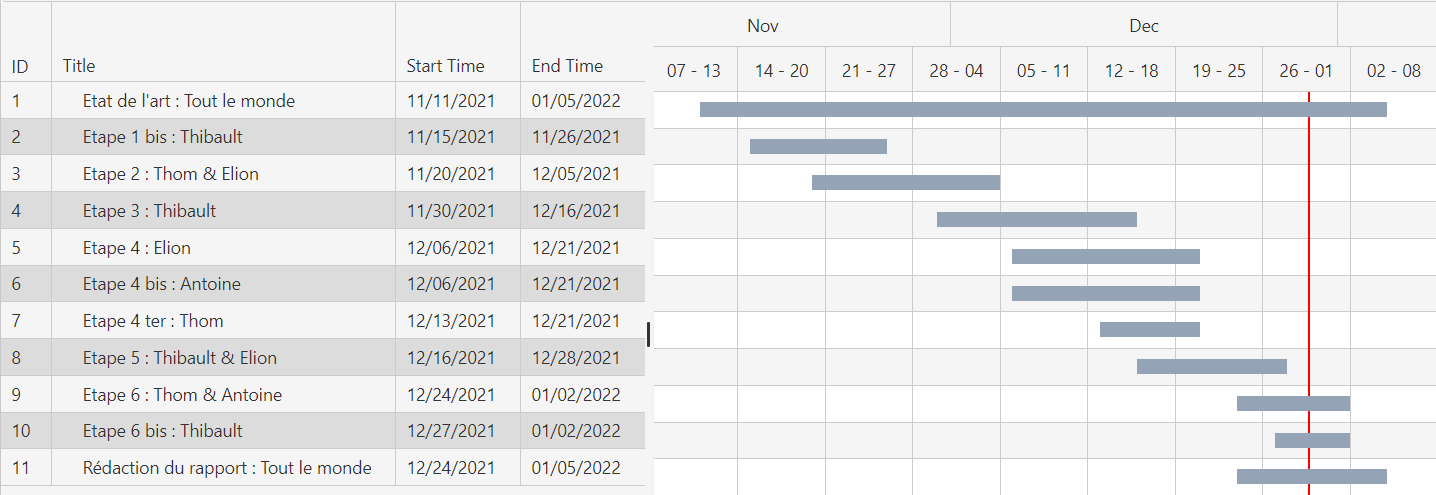
\includegraphics[scale = 0.575] {Gantt.png}
        \caption{Diagramme de Gantt (dernière version : 29/12/2021)}
        \label{fig:gantt}
    \end{figure}

\newpage
\subsection{Outils de Travail}
\noindent
Nous avons utilisé le répertoire Git fourni par l'école durant tout le projet, chaque membre du groupe avait sa propre branche dans laquelle chacun mettait son travail réalisé. Thibault gérait la branche master, avec la fusion des branches.

\subsection{Comptes-rendu des réunions}
    
    \subsubsection{9 novembre 2021}
    \vskip 0.75cm

\begin{center}
\begin{tabular}[]{|l|l|}
     \hline 
     Présent & Absent\\
     \hline
     Cheneviere Thibault &\\ Guillot Thom & \\
     Hashani Elion &\\ Yebouet Antoine &\\
     \hline
\end{tabular}
\end{center}

\vskip 0,75cm

\noindent
\textbf{Ordre du jour}

\begin{enumerate}
    \item Proposer des idées pour l'application 
\end{enumerate}

\vskip 0.75cm

\noindent
\textbf{Idées}

\noindent
\textit{Idées proposées par l'ensemble de l'équipe projet : }
    
    \begin{itemize}
        \item Trouver un moyen d’attirer les gens à voter (aller chercher les gens chez eux pour les faires voter)
        \item Sondage, 1 vote par compte (système de vérification des comptes avec unicité de la personne, par exemple système de vérification de carte d’identité). Espace avec échange d’idées (commentaire, …)
        \item Espace avec les news de la ville (politique, divers, sport, …)
        \item Compte avec des accès spécifiques (Maire, conseil municipal, admin, citoyen, …)
        \item Système de notification avec des mails, messages ou autre
        \item Système de lien avec les flux sociaux des politiciens
        \item Résumé de tous les programmes des différents partis/candidats.
        \item Faire une interface attrayante, interactive et qui attire les personnes à venir lire les informations.
        \item Faire un camembert des capacités sur 5 sujets et les personnes peuvent donner leur avis sur chaque candidat après avoir lu leur programme.
        \item Faire une interface avec un hémicycle sur lequel on peut directement cliquer pour avoir accès aux informations des candidats suivant leurs orientations politiques.
    
    \end{itemize}
 
\vskip 1cm
\noindent
\textit{TO DO LIST}
\vskip 0.25cm

\begin{itemize}
    \item Chercher des exemples et des applications de Civic Tech.
    \itemÉtablir ensuite un ensemble de critères que l’on veut avoir sur notre application.
\end{itemize}


    
    \newpage
    \subsubsection{19 novembre 2021}
    \vskip 0.75cm

\begin{center}
\begin{tabular}[]{|l|l|}
     \hline 
     Présent & Absent\\
     \hline
     Cheneviere Thibault & Guillot Thom\\ 
     Hashani Elion &\\ Yebouet Antoine &\\
     \hline
\end{tabular}
\end{center}


\vskip 0,75cm

\noindent
\textbf{Ordre du jour}

\begin{enumerate}
    \item Objectif
    \item Avancement du projet
\end{enumerate}

\vskip 0.5cm

\noindent
\textbf{Objectif}\\
\noindent
La séance d'aujourd'hui a pour but de déterminer les fonctionnalités du projet que l'on souhaite implémenter et obtenir une validation de la part des responsables du module. \\ 

\noindent
\textit{Fonctions principales}
\begin{itemize}
    \item Page de News de la ville (en page d'accueil) avec les news des clubs de la ville (sportif, artistique, culturel, …), nouvelle décision des élus (projets qui ont été acceptés).
    \item Système d’aide à la prise de décision : avant de voter un projet, permettre au citoyen de choisir le budget alloué à ce projet, impliquer les citoyens sur les plans urbains de la ville à travers des sondages (les mineurs ne pourront pas voter et il y a un vote unique par personne) et des discussions. 
    \item Système lors d'élection : présenter les programmes des différents candidats à travers un hémicycle (représentation graphique) qui répertorie tous les candidats. Les candidats écriront directement leur programme pour éviter les informations biaisées.
    \item Système d’entraide entre les riverains : faire une plateforme pour poster ses annonces pour demander de l’aide ou proposer son aide (par exemple aide pour faire du bricolage, de la mécanique, aide sur un problème avec du matériel informatique, …)
    \item Système de création de projet par les citoyens : système de budget participatif (possibilité de financer des projets de riverains) et possibilité de promouvoir un projet avec des pétitions pour les faire connaître et financer par les élues.
    \item Système de signalisation des problèmes : chaque citoyen peut signaler des incivilités ou des problèmes liés à la gestion de la ville (problème de circulation sur certains axes, problème de ramassage des poubelles dans certains quartiers, …)

\end{itemize}

\vskip 0.5cm

\noindent
\textbf{Avancement du projet}

\vskip 0.25cm
\noindent
\textit{Etape 1 bis :} \\
Thibault a commencé l'implémentation du login/authentification des candidats.
\\Elion a débuté la rédaction de la charte de projet, accompagné de la gestion du document.

\vskip 0.25cm

\noindent
\textit{Etat de l'art :}
\\Nous avons trouvé plusieurs exemples de la Civic Tech et ses exemples d'implémentations 

\vskip 1cm
\noindent
\textit{TO DO LIST}
\vskip 0.25cm

\begin{itemize}
\item Pour tous :
\begin{itemize}
    \item Attendre la réponse des responsables du modules pour démarrer l'implémentation
    \item Continuer la recherche sur la Civic Tech
    \item Réaliser la matrice SWOT
\end{itemize}
\item Pour Elion :
\begin{itemize}
    \item Terminer la charte et la gestion du document
\end{itemize}
\item Pour Thibault :
\begin{itemize}
    \item Terminer le système de login
\end{itemize}
\end{itemize}
    
    \newpage
    \subsubsection{24 novembre 2021}
    \vskip 0.75cm

\begin{center}
\begin{tabular}[]{|l|l|}
     \hline 
     Présent & Absent\\
     \hline
     Cheneviere Thibault & Yebouet Antoine\\ 
     Guillot Thom &\\ Hashani Elion &\\
     \hline
\end{tabular}
\end{center}


\vskip 0,75cm

\noindent
\textbf{Ordre du jour}

\begin{enumerate}
    \item Objectif
    \item Avancement du projet
    \item Description de l'application
\end{enumerate}

\vskip 0.25cm

\noindent
\textbf{Objectif}\\
\noindent
La séance d'aujourd'hui a pour but de clarifier la description de l’application avec les retours fait sur la première proposition. \\ 

\noindent
\textit{Objectif de l'application :}\\
L’objectif de l’application est de faciliter le vote en donnant un accès facile au programme de chaque candidat et en proposant une première analyse du programme qui pourra être affinée par les citoyens les plus investis. Ensuite la localisation des différents bureaux de vote facilite la démarche de vote pour les personnes les plus récalcitrantes.

\vskip 0.25cm

\noindent
\textbf{Avancement du projet}\\
\noindent
\textit{Etape 1 bis :} \\
Thibault a terminé l'implémentation du login/authentification des candidats.
\\Elion a fini la rédaction de la charte de projet et ainsi que celle de la gestion du document et ajoute les étapes du projet au fur et à mesure. Matrice SWOT réalisé.

\vskip 0.25cm

\noindent
\textit{Etape 2 :}\\
Thom a commencé à réaliser la page d'accueil du site

\vskip 0.25cm

\noindent
\textbf{Description de l'application}
\begin{itemize}
    \item Chaque candidat aura des identifiants pour pouvoir se connecter et entrer son programme en ligne.
    \item Ensuite après le référencement d’un programme, une analyse automatique permet de « noter » suivant plusieurs critères le candidats (critère écologique, sociale, économique). Cette notation permet ensuite d’afficher 3 barres sur le site internet plus ou moins rempli (pourcentage de remplissage).
    \item Chaque citoyen peut ensuite influer sur ces notations (dans la limite d’une variation de $\pm 5\%$) après avoir lu le programme d’un candidat (permet d’avoir un avis plus large sur la perception du candidat).
    \item Système de localisation des différents bureaux de vote pour faciliter le vote de chacun
\end{itemize}

\vskip 1cm
\noindent
\textit{TO DO LIST}
\vskip 0.25cm

\begin{itemize}
    \item Continuer la recherche sur la Civic Tech sur des algorithmes déjà existants
    \item Finir l'étape 2
    \item Entamer l'étape 3
    \item Réaliser le Gantt
\end{itemize}
    
    \newpage
    \subsubsection{30 novembre 2021}
    \vskip 0.75cm

\begin{center}
\begin{tabular}[]{|l|l|}
     \hline 
     Présent & Absent\\
     \hline
     Cheneviere Thibault &\\ Guillot Thom & \\
     Hashani Elion &\\ Yebouet Antoine &\\
     \hline
\end{tabular}
\end{center}

\vskip 0,75cm

\noindent
\textbf{Ordre du jour}

\begin{enumerate}
    \item Objectif
    \item Avancement du projet
    \item Description et attribution des work packages
\end{enumerate}

\vskip 0.25cm

\noindent
\textbf{Objectif}\\
\noindent
La séance d'aujourd'hui a pour but de répartir les tâches à effectuer sur le projet ainsi que de lancer les différentes tâches.

\vskip 0.25cm

\noindent
\textbf{Avancement du projet}

\noindent
\textit{Etape 2 :} \\
Thom a quasiment terminé la page d'accueil du site, il ne reste plus que l'esthétique de la page. Les rubriques "Comment ça marche ?" et "Liste des candidats" sont entamés\\
Elion a réalisé le Gantt en adéquation avec les demandes des membres du groupe et a débuté une matrice RACI

\vskip 0.25cm

\noindent
\textit{Etape 3 :}\\
Thibault a bien entamé le programme portant sur l'analyse des programmes des candidats par mots-clés. Chaque mot-clé a un ordre d'importance et cela permettra de mieux noter le programme d'un candidat

\vskip 0.25cm

\noindent
\textbf{Description et attribution des work packages}
\begin{itemize}
    \item Pour Thibault :
\begin{itemize}
    \item Terminer le système de notation des programmes par mots-clés (utilisation d’un dictionnaire pondéré par critère pour noter le programme) (\textit{Etape 3})
\end{itemize}
\end{itemize}
\begin{itemize}
    \item Pour Thom :
\begin{itemize}
    \item Finir la page home avec une explication du fonctionnement du site et un exemple pour se familiariser avec le système de notation, la rendre ludique. (\textit{Etape 4 ter})
\end{itemize}
\end{itemize}
\begin{itemize}
    \item Pour Elion :
\begin{itemize}
    \item Nouveau jalonnement dans la charte, effectuer la matrice RACI avec les work packages suivant.
    \item Commencer l'analyse des listes des candidats (\textit{Etape 4})
\end{itemize}
\end{itemize}
\begin{itemize}
    \item Pour Antoine :
\begin{itemize}
    \item Faire l’interface d’affichage des programme (liste de tous les programmes en grid) et affichage du programme détaillé avec les membres de la liste et les différentes notation du programme (\textit{Etape 4 bis})
\end{itemize}
\end{itemize}
\begin{itemize}
    \item A réaliser après avoir terminé les work packages attribués :
\begin{itemize}
    \item Faire l’interface utilisateur pour modifier la note d’un programme sur le site (vérifier que l’utilisateur a lu le programme, et modification unique de la note du programme) (\textit{Etape 6 bis})
    \item Faire la page avec l'hémicycle : hémicycle statique avec en dessous en colonne en dessous de la tendance politique la liste des candidats cliquable pour arriver sur leur programme (faire des sortes de carte pour les candidats avec leur photo, nom, notations dans les différents domaines, parti politique)
    \item Système de localisation du bureau de vote le plus proche (par form en demandant l’adresse de la personne ou en utilisant l’adresse IP) (\textit{Etape 6})
\end{itemize}
\end{itemize}

\vskip 1cm
\noindent
\textit{TO DO LIST}
\vskip 0.25cm

\begin{itemize}
    \item Chacun avance/termine son work package
    \item Recherche sur la Civic Tech
\end{itemize}


    
    \newpage
    \subsubsection{16 décembre 2021}
    \vskip 0.75cm

\begin{center}
\begin{tabular}[]{|l|l|}
     \hline 
     Présent & Absent\\
     \hline
     Cheneviere Thibault & Yebouet Antoine\\ 
     Guillot Thom &\\ Hashani Elion &\\
     \hline
\end{tabular}
\end{center}


\vskip 0,75cm

\noindent
\textbf{Ordre du jour}

\begin{enumerate}
    \item Objectif
    \item Avancement du projet
    \item Nouveaux objectifs pour le groupe
\end{enumerate}

\vskip 0.25cm

\noindent
\textbf{Objectif}\\
\noindent
La séance d'aujourd'hui a pour but de :
\begin{itemize}
    \item Fixer des nouveaux objectifs pour la semaine
    \item Faire un point sur l’avancement des objectifs pris
\end{itemize}

\vskip 0.25cm

\noindent
\textbf{Avancement du projet}\\
\noindent
\textit{Etape 3 :}\\
Partie de notation des programmes terminées, on peut encore compléter cette partie en référençant plus de mots clés.
 
\vskip 0.25cm
\noindent
\textit{Etape 4 :}\\
Charte de projet modifiée avec les nouveaux jalonnements et à jour.\\
Etude des listes non réalisée.

\vskip 0.25cm
\noindent
\textit{Etape 4 bis :}\\
Bien avancée, mais quelques détails à régler notamment l'affichage des membres de la liste.

\vskip 0.25cm
\noindent
\textit{Etape 4 ter :}\\
Page d’accueil : forme de la page d’accueil terminée, il reste les champs à compléter,la liaison avec la base de données pour la page liste des candidats

\vskip 0.25cm

\noindent
\textbf{Nouveaux objectifs pour le groupe}
\begin{itemize}
    \item Pour Antoine :
\begin{itemize}
    \item Finir la page d'affichage des programmes (\textit{Etape 4 bis})
\end{itemize}
\end{itemize}
\begin{itemize}
    \item Pour Elion :
\begin{itemize}
    \item Faire la page de référencement de la liste des membres (sur la page de référencement du programme on ajoute une partie pour ajouter les membres d’une liste). (\textit{Etape 4})
    \item Faire l’étude de la répartition des catégorie sociaux-professionnelles dans une liste (\textit{Etape 4})
\end{itemize}
\end{itemize}
\begin{itemize}
    \item Pour Thibault :
\begin{itemize}
    \item Faire les cartes pour les candidats (affichage de la photo, nom prénom, phrase d’accroche et barre de notation suivant les critères) (\textit{Etape 5})
    \item Faire l’interface utilisateur pour modifier la note d’un programme. (\textit{Etape 6 bis})
\end{itemize}
\end{itemize}
\begin{itemize}
    \item Pour Thom :
\begin{itemize}
    \item Faire la partie liste de candidats avec la partie hémicycle avec l’affichage des candidats en dessous. (\textit{Etape 4 ter})
    \item Finir d’écrire la partie « Comment ça marche ? » (\textit{Etape 4 ter})
\end{itemize}
\end{itemize}

\vskip 1cm
\noindent
\textit{TO DO LIST}
\vskip 0.25cm

\begin{itemize}
    \item Commencer à réaliser des tests sur les fonctions python 
    \item Chacun avance/termine son work package
    \item Recherche sur la Civic Tech
\end{itemize}

    \newpage
    \subsubsection{26 décembre 2021}
    \vskip 0.75cm

\begin{center}
\begin{tabular}[]{|l|l|}
     \hline 
     Présent & Absent\\
     \hline
     Cheneviere Thibault &\\ Guillot Thom & \\
     Hashani Elion &\\ Yebouet Antoine &\\
     \hline
\end{tabular}
\end{center}

\vskip 0,75cm

\noindent
\textbf{Ordre du jour}

\begin{enumerate}
    \item Objectif
    \item Avancement du projet
    \item Nouvelles tâches
\end{enumerate}

\vskip 0.25cm

\noindent
\textbf{Objectif}\\
\noindent
La séance d'aujourd'hui a pour but d'effectuer un jalonnement pour observer le travail effectué pendant ces vacances ainsi que d'attribuer de nouvelles tâches à chacun.

\vskip 0.25cm

\noindent
\textbf{Avancement du projet}

\noindent
\textit{Etape 4 :}\\
Page de référencement de la liste des membres faite, ainsi que l’étude des catégories socio-professionnelles des listes

\vskip 0.25cm

\noindent
\textit{Etape 4 bis :}\\
La page est opérationnelle et affiche bien tous les changements faites par le candidat, reste plus qu’à afficher les votes des utilisateurs.

\vskip 0.25cm

\noindent
\textit{Etape 4 ter :}\\
Page d’accueil : les champs à compléter sont terminés ,la liaison avec la base de données pour la page liste des candidats est faite. La partie “Comment ça marche ?” est aussi terminé.

\vskip 0.25cm

\noindent
\textit{Etape 5 :}\\
Cartes représentant les candidats sont réalisées.

\vskip 0.25cm

\noindent
\textit{Etape 6 bis :}\\
L’interface utilisateur pour modifier est entamée.

\vskip 0.25cm

\noindent
\textit{Tests :}\\
Des tests ont été effectués sur quelques fonctions python aboutissant à des résultats positifs. 

\vskip 0.25cm

\noindent
\textbf{Nouvelles tâches}
\begin{itemize}
    \item Commencer la rédaction du rapport
    \item Terminer les étapes 5,6 et 6 bis
    \item Rédiger d'autres tests sur les fonctions python restantes
\end{itemize}

\vskip 0.75cm
\noindent
\textit{TO DO LIST}
\vskip 0.25cm

\begin{itemize}
    \item OBLIGATOIREMENT : Faire les nouvelles tâches avant la prochaine réunion 
    \item Recherche sur la Civic Tech
\end{itemize}
%Fin chapitre 5

\newpage
%Debut chapitre 6 : Bilan du projet
\section{Bilan du projet}
\vskip 0.60cm
\subsection{Bilan global du projet}
\vskip 0.25cm
\noindent
\begin{tabularx}{\textwidth}{|X|X|}
    \hline 
    Travail attendu & Travail réalisé \\
    \hline
    Faciliter la démocratie participative locale en prenant en compte les services déjà proposés par la Civic Tech afin de proposer une innovation dans ce domaine. Le but est de s'appuyer sur les outils donnés au cours de l'année : une application web, du code Python et une base de données.
    & 
    Application web qui répertorie chaque candidat inscrits aux élections locales sous forme de cartes contenant des informations avec lesquelles peuvent intéragir de simples visiteurs. Les cartes synthétisent l'attention que porte le candidat sur différents thèmes afin de faciliter le choix de vote. Une intéraction sur ces statistiques est possible afin de mieux correspondre à la vision qu'ont les visiteurs sur le candidat en question.
    \\
    \hline
\end{tabularx}
\vskip 0.60cm
\noindent
\begin{tabularx}{\textwidth}{|X|X|X|}
    \hline
     & Points positifs & Points négatifs \\
    \hline
    \textbf{Écriture du code} & 
    Python est un des langages les plus utilisés de nos jours ce qui facilite grandement la recherche d'informations et de solutions concernant le code. Python est intuitif et très compréhensible de par son système d'indentation.
    \vskip 0.25cm
    HTML, CSS et Bootstrap 5 sont pratiques pour la création de site et sont facilement reliables à Python grâce à des outils comme Flask.
    \vskip 0.25cm
    La base de donnée est facilement accessible grâce à SQLite3 en python ce qui permet l'utilisation directe des informations dans les fonctions Python créées pour le bon fonctionnement du site.
    &
    HTML, CSS et Bootstrap 5 sont très spécifiques quand il s'agit de la mise en page du site en lui-même ce qui rend les codes longs et compliqués à mettre en place.
    \vskip 0.25cm
    La base de donnée possède de nombreuses relations de dépendance et il peut souvent arriver d'oublier de relier certaines informations. Il faut donc souvent y faire attention et cela complique la manipulation de celle-ci.
    \\
    \hline
\end{tabularx}
\vskip 0.60cm
\subsection{Bilan du projet par membre}
\vskip 0.25cm
\subsubsection{Cheneviere Thibault}
\noindent
\begin{tabularx}{\textwidth}{|X|X|}
    \hline
    \textbf{Points positifs} & {Nous avions un groupe avec une bonne ambiance et de bonnes idées ce qui a permis de trouver un sujet intéressant et original.} \\
    \hline
    \textbf{Points négatifs} & {Je pense qu'il y a eu un manque de communication au niveau de la répartition du travail ce qui a impacté la performance du groupe.} \\
    \hline
    \textbf{Expérience personnelle} & {J'ai pu mettre en oeuvre les techniques de python, de web et de base de données vues en cours mais aussi réutiliser des notions que j'avais vu avant ce projet. De plus, c'était ma première expérience de travail en groupe sur un projet informatique et je pense que cela me permettra d'améliorer mon approche et mon travail sur les autres projets.} \\
    \hline
    \textbf{Axes d'amélioration} & {Comme je l'ai dit dans les points négatifs, je pense qu'une meilleure communication ainsi qu'une meilleure répartition du travail permettraient de rendre les prochains projets encore meilleurs.} \\
    \hline
\end{tabularx}
\subsubsection{Guillot Thom}
\noindent
\begin{tabularx}{\textwidth}{|X|X|}
    \hline
    \textbf{Points positifs} & Les idées de chacun étaient pertinentes, à la fois pour implémenter de nouvelles fonctionnalités, mais aussi pour corriger/améliorer une déjà existante. L'ambiance du groupe a permis de travailler dans un climat de bonne entente.\\
    \hline
    \textbf{Points négatifs} & La répartition du travail a été difficile, notamment avec la période de vacances qui nous a séparé et nous n'avions pas les mêmes plages horaires pour travailler.\\
    \hline
    \textbf{Expérience personnelle} & J'ai enrichi ma compréhension en HTML, CSS, Bootstrap 5, JavaScript et Python avec les codes que j'ai pu écrire, mais aussi en regardant le fonctionnement des algorithmes de mes camarades.\\
    \hline
    \textbf{Axes d'amélioration} & Il faudrait à l'avenir améliorer la communication et l'évaluation de la faisabilité et la pertinence d'une idée.\\
    \hline
\end{tabularx}
\subsubsection{Hashani Elion}
\noindent
\begin{tabularx}{\textwidth}{|X|X|}
    \hline
    \textbf{Points positifs} & Le groupe était agréable, nous avons su développer plusieurs idées sur le projet. La bonne ambiance ainsi que les idées pertinentes proposées nous ont permis de bien travailler.  \\
    \hline
    \textbf{Points négatifs} & J'ai trouvé que l'on avait mis trop de temps à se répartir les tâches et donc à vraiment se plonger dans le projet.\\
    \hline
    \textbf{Expérience personnelle} & Ce projet m'a permis de découvrir et surtout de comprendre le fonctionnement d'une application, j'ai pu m'excercer et donc m'améliorer dans les différents langages de programmation.\\
    \hline
    \textbf{Axes d'amélioration} & Renforcer davantage la communication pour que tous les membres soient plus impliqués et surtout pour que le projet avance de manière régulière. \\
    \hline
\end{tabularx}
\subsubsection{Yebouet Antoine}
\noindent
\begin{tabularx}{\textwidth}{|X|X|}
    \hline
    \textbf{Points positifs} & Les idées se sont vite construites dans l'équipe et l'ambiance était bonne. La motivation était présente jusqu'au bout.\\
    \hline
    \textbf{Points négatifs} &  Après la phase initiale du projet, il y a eu un manque de communication en ce qui concerne la répartition des tâches.\\
    \hline
    \textbf{Expérience personnelle} & Ce projet m'a permis de bien cerner les concepts et la technique en ce qui concerne la réalisation d'une application Web, dans les 3 volets concernés, et j'ai amélioré mes connaissances dans les langages utilisés.\\
    \hline
    \textbf{Axes d'amélioration} & Améliorer la communication au sein du groupe et aussi une meilleure prise d'initiative en ce qui me concerne.\\
    \hline
\end{tabularx}
\vskip 0.60cm
%Fin chapitre 6

\appendix

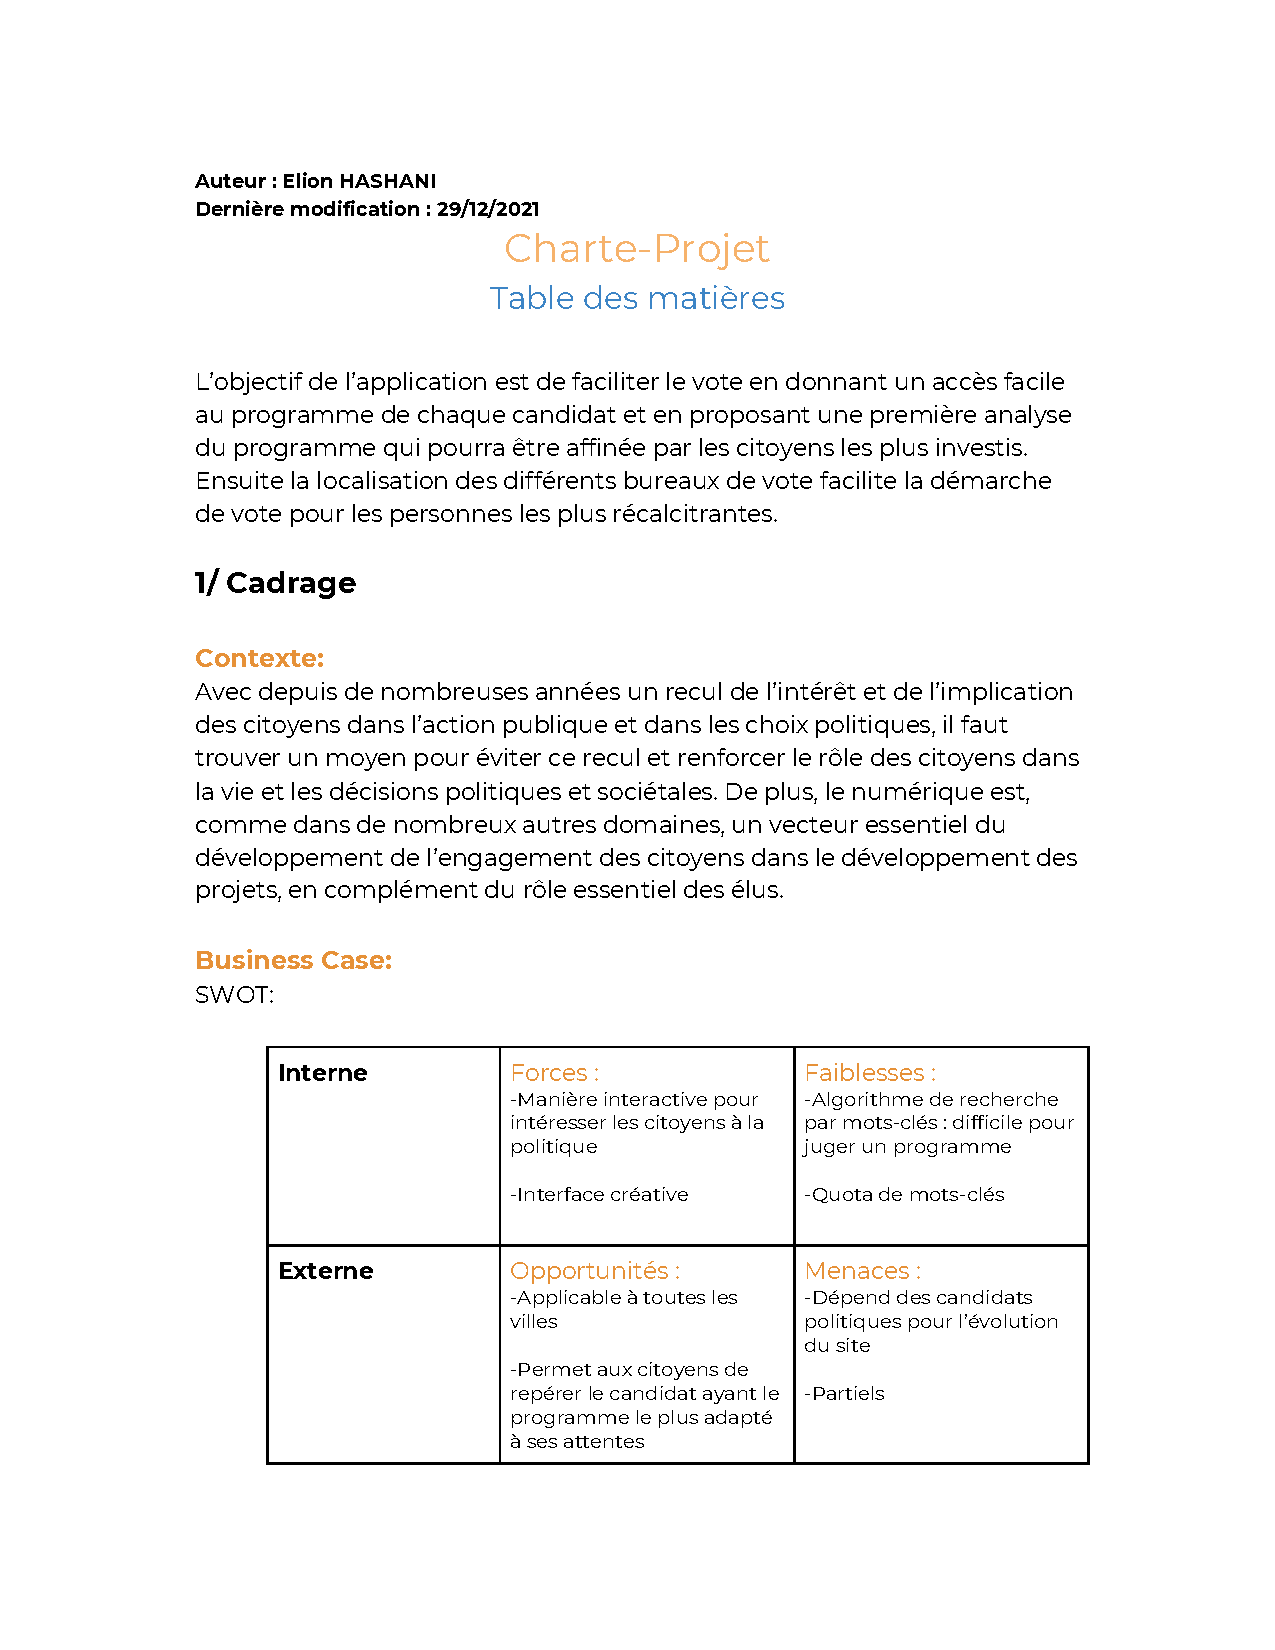
\includepdf[pages=-, pagecommand=\textbf{\huge Annexe}]{Charte Projet.pdf}
\end{document}